\section{Results}
\begin{figure}[h]
    \centering 
    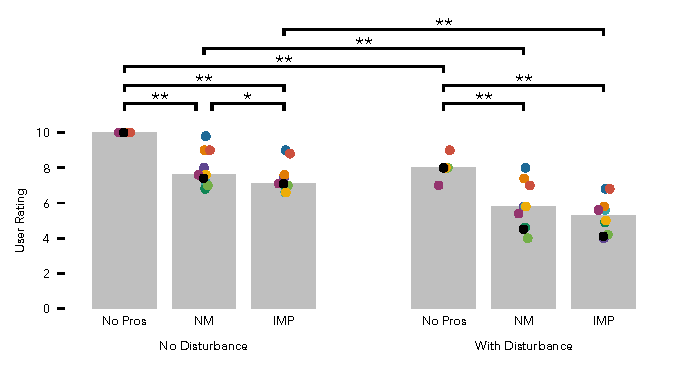
\includegraphics[width=\textwidth]{treadmill_vib_user_scores}
    \caption{Average user ratings across all trials in both the undisturbed and
    disturbed walking conditions when walking without the prosthesis (No Pros)
    and with the Neuromuscular (NM) prosthesis control and impedance (IMP)
    prosthesis control. Grey bars show the mean across subjects.  Statistical
    significance assessed by Welch's $t$-test. $*$:~$p < 0.05$, $**$:~$p <
    0.01$, $***$:~$p < 0.001$.}\label{fig:treadmill_user_ratings}
\end{figure}

\begin{figure}[h]
    \centering 
    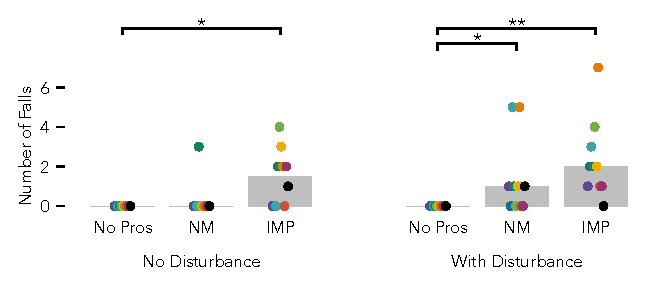
\includegraphics[width=\textwidth]{treadmill_vib_num_falls}
    \caption{Total number of falls across all trials in both the undisturbed and
    disturbed walking conditions when walking without the prosthesis (No Pros)
    and with the Neuromuscular (NM) prosthesis control and impedance (IMP)
    prosthesis control. Grey bars show the median number of falls across all
    subjects. Statistical significance assessed by Mann-Whitney $U$ test.
    $*$:~$p < 0.05$, $**$:~$p < 0.01$.}\label{fig:treadmill_exp_falls}
\end{figure}

\begin{table}[h]
  \begin{center}
    \begin{tabular}{lcc}
      Fall Types & Neuromuscular & Impedance \\
      \midrule
      Fall Forward &  1 &  0 \\
      Fall Backwards &  6 &  4 \\
      Fall Left &  1 &  0 \\
      Fall Right &  0 &  3 \\
      Missed Stance / Swing Transition &  3 &  0 \\
      Missed Stance 2 / Stance 3 Transition &  0 &  7 \\
      Knee Collapse & 0 & 15 \\
      Swing Trip & 4 & 12 \\
    \end{tabular}
  \end{center}
  \caption{Tally of observed reasons for falls across all subjects and across
  both the undisturbed and disturbed walking conditions. Falls were manually
  classified based on video and logged prosthesis data. An individual Fall can
  be assigned more than one reason.}\label{tab:treadmill_exp_fall_reasons}
\end{table}

\begin{figure}[h]
    \centering 
    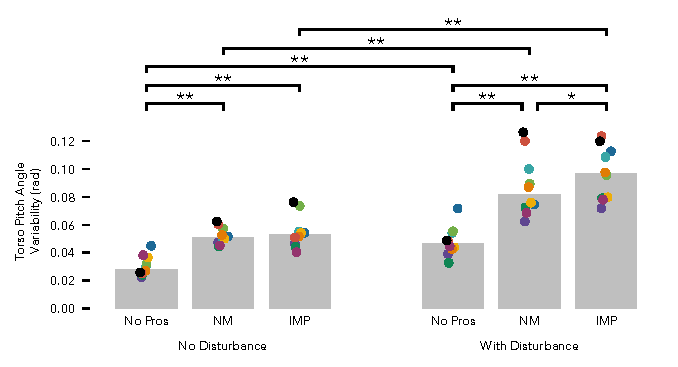
\includegraphics[width=\textwidth]{treadmill_vib_torso_var_x}
    \caption{Torso pitch angle variation. Angle variation calculated as the
    interquartile range of torso angles after the median torso angle trajectory
    over the strides in a trial is subtracted out. For the prosthesis trials, we
    report the average variation across the five trials for each condition.
    Grey bars show the mean across subjects.  Statistical significance assessed
    by Welch's $t$-test. $*$:~$p < 0.05$, $***$:~$p <
    0.001$.}\label{fig:treadmill_exp_torso_var_x}
\end{figure}

\begin{figure}[h]
    \centering 
    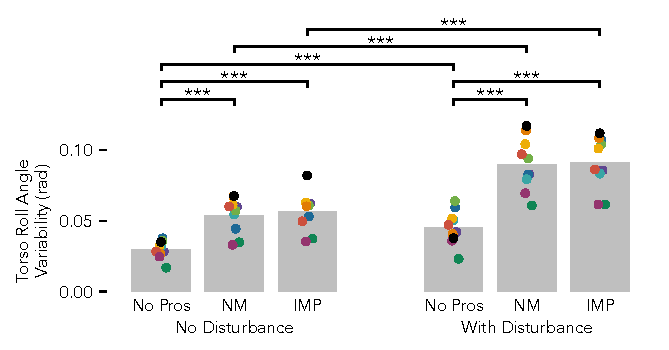
\includegraphics[width=\textwidth]{treadmill_vib_torso_var_y}
    \caption{Torso roll angle variation. Angle variation calculated as the inter
    quartile range of torso angles after the median torso angle trajectory over
    the strides in a trial is subtracted out. For the prosthesis trials, we
    report the average variation across the five trials for each condition.
    Grey bars show the mean across subjects.  Statistical significance assessed
    by Welch's $t$-test.$***$:~$p < 0.001$.}\label{fig:treadmill_exp_torso_var_y}
\end{figure}

\begin{figure}[h]
    \centering 
    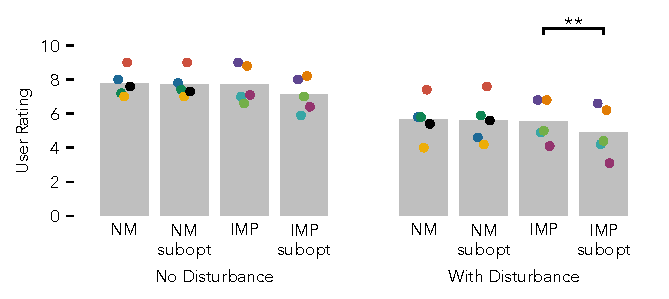
\includegraphics[width=\textwidth]{treadmill_vib_user_scores_subopt}
    \caption{Comparison of user scores of optimal versus suboptimal parameters
    for the neuromuscular and impedance control strategies. Grey bars show the
    mean user rating across subjects. Statistical significance assessed by
    Welch's $t$-test. $**$:~$p <
    0.01$.}\label{fig:treadmill_exp_user_ratings_subopt}
\end{figure}

\begin{figure}[h]
    \centering 
    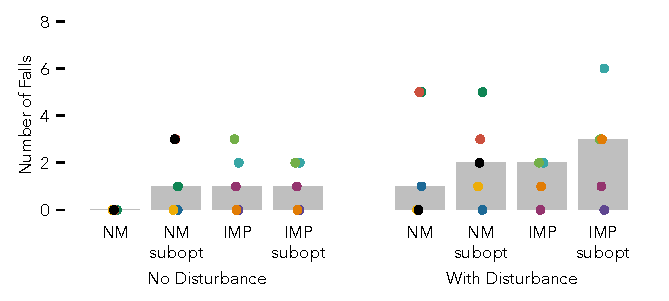
\includegraphics[width=\textwidth]{treadmill_vib_num_falls_subopt}
    \caption{Comparison of number of falls of optimal versus suboptimal
    parameters for the neuromuscular and impedance control strategies. Grey bars
    show the median number of falls across subjects. Statistical significance
    assessed by Mann-Whitney $U$
    test.}\label{fig:treadmill_exp_user_ratings_subopt}
\end{figure}

\begin{marginfigure}
    \centering 
    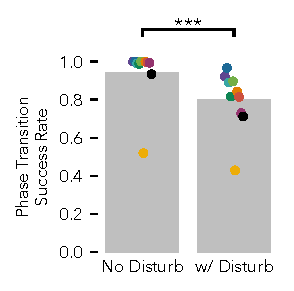
\includegraphics[width=\textwidth]{phase_success}
    \caption{Fraction of steps for which impedance control successfully
    transitions through all three stance phases. Introduction of gait
    disturbances significantly decreases the transition success rate. Grey bars
    show the mean success rate across all users. Statistical significance
    assessed by Welch's $t$-test. $***$:~$p <
    0.001$.}\label{fig:treadmill_exp_phase_success}
\end{marginfigure}
